\chapter{Introduction}
\label{ch:introduction}

Ever since the camera and phone were unified into smartphones, we have seen an increasing interest for image understanding (specifically to identify the content of an image) but text recognition still faces challenges within images of unstructured scenes. While successes in character recognition have a long history with \gls{ocr} engines \citep{Smith:1987tg}, these are typically applied under strict conditions (e.g., flatbed scanners for documents without distracting backgrounds). Once applied within the context of a natural scene, real-world discrepancies pose serious shortcomings, such as illumination and viewpoint conditions, blur and glare variations, geometric and photometric distortion, and differences in font size and style \citep{Zhang:2008vfa, Jung:2004uw}. Overcoming these issues has motivated a variety of different techniques in order to realise potential applications that make use of text recognition at scale.

With the ubiquity of smartphone cameras, practical applications of natural image processing have increased. In the last two decades, we have seen the development of point-and-shoot product recognition \citep{Tsai:2010cn,Girod:2011gw}, object detection in videos \citep{Sivic:2003tj}, building recognition \citep{Takacs:2008cg}, image feature extraction to improve visual-based search engines \citep{Lowe:2004kp,Bay:2008ud}, and translation services of American Sign Language gestures \citep{Jin:2016jd}. Nonetheless, embedded text within images contains indexable data on the image's semantics \citep{Smeulders:2000tx}; if text extraction is therefore not robust, information extraction suffers.

Text detection robustness is a factor which severely limits a text recognition pipeline. Research in overcoming such limitations have been competed numerous competitions \citep{Lucas:2003iw, Lucas:2005bq, Shahab:2011hq, Hua:2004vf}, where robustness is the key focus in the image processing pipelines proposed. This focus was reiterated by \citet{Chen:2011ul}, who state the primary prerequisite for text-based recognition (especially within natural scenes) is the text location must be robustly located.

As with any data processing pipeline, false negatives increase where early stages of the pipeline fail, and therefore detection of these potential candidates must be robust. We can reduce errors in a pipeline where: (1) there may be unwarranted stages of the pipeline, and therefore \textit{excluding} unnecessary stages may also assist in reducing error cases, and (2) by piping through unmatched candidates to further pipelines, which can increase the detection. Both guide in improving robust detection, and this is therefore a key consideration made in our assessment of how useful that pipeline may be. Without the construct of robustness, we restrict these pipelines to very confined conditions, and its usefulness in products is not warranted.

\section{Background}
\label{sec:introduction:background}

This study focuses on character recognition in unstructured scenes (Figure~\ref{fig:sample_rbns}): specifically, short, alphanumeric number sequences. Previous works present methods to extract these sequences in various areas, namely: License Plate Recognition (LPR\newacronym{lpr}{LPR}{Licence Plate Recognition}) systems \citep{CanoPerez:2003fq,Anagnostopoulos:2006wv}; Traffic Sign Recognition (TSR\newacronym{tsr}{TSR}{Traffic Sign Recognition}) \citep{Eichner:2008dw,Kundu:2015vq,Seo:2015ez,Lian:2016dc}; and, street number recognition, specifically a study by \citet{Netzer:2011to}, using Google Street View\footnoteurl{https://www.google.com/streetview/}{13 May 2017} to determine the numerical value of street numbers. Figure~\ref{fig:sample_sequences} highlights typical usage of these sequences.

Different applications apply varying methods to parse short alphanumeric characters. There are typically two stages of any parsing method: \textit{detection} and \textit{recognition}. Detection refers to locating possible candidates and recognition refers to the representation of the text itself. Detection techniques usually are categorised as either connected component (CC)\newacronym{cc}{CC}{Connected Component}-based or learning or texture-based. CC-based detection will typically use a set of distinct properties on the image to detect relevant areas (such as width, stroke and colour) while learning-based feed images into a classifier that can distinguish candidates from false positives. The recognition phase can typically be achieved using optical image recognition OCR engines (such as Tesseract\footnoteurl{https://github.com/tesseract-ocr/tesseract}{14 May 2017}), machine learning algorithms or deep neural networks (NNs\newacronym{nn}{NN}{Neural Network}) to classify the detected regions. % TODO: Find citation

{
  \itshape
  This study proposes the development of a learning-based detection and recognition pipeline using deep-learning neural networks within the context of unstructured photos, with a focus on marathon Racing Bib Numbers (RBNs)\newacronym{rbn}{RBN}{Racing Bib Number}, as shown in Figure~\ref{fig:sample_rbns}.
}

\newpage
\begin{figure}[h!]
  \centering
  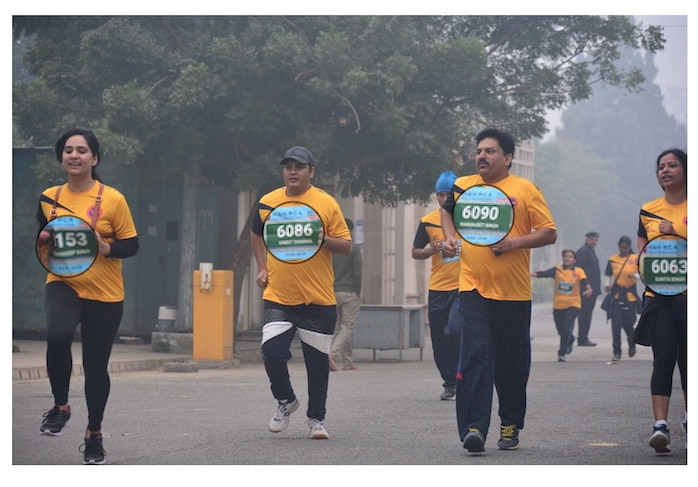
\includegraphics[width=0.7\textwidth]{images/introduction/rbn}
  \caption[Sample racing bib numbers]{Four RBNs in a sample marathon photo.}
  \label{fig:sample_rbns}
\end{figure}
\vspace{\fill}
\begin{figure}[h!]
  \centering
  \begin{subfigure}[b]{0.4\textwidth}
    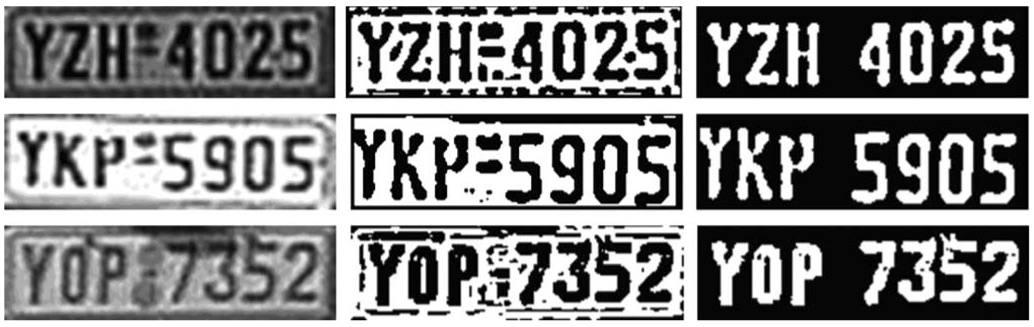
\includegraphics[width=\textwidth]{images/introduction/lpr}
    \caption{\footnotesize Successful LPR character segmentation \citep{Anagnostopoulos:2006wv}. \textit{Left to right}: original image; region segmentation; character segmentation after negation, height and orientation measurements.}
  \end{subfigure}
  \hspace{0.05\textwidth}
  \begin{subfigure}[b]{0.4\textwidth}
    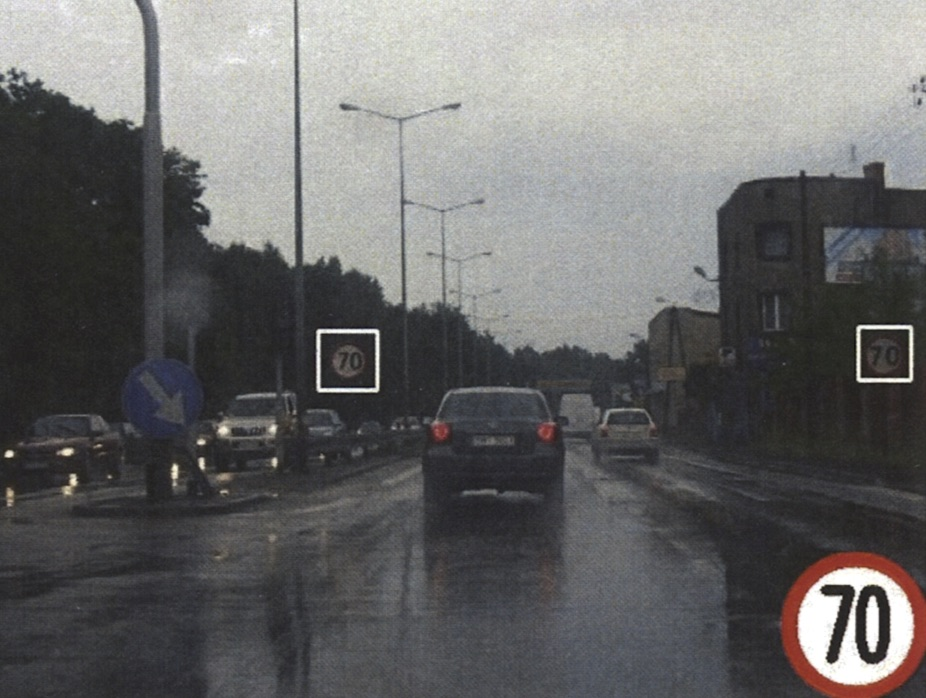
\includegraphics[width=\textwidth]{images/introduction/tsr}
    \caption{\footnotesize Successful recognition of speed sign digits shown in \citet{Eichner:2008dw}.}
  \end{subfigure}\\
  \vspace{1cm}
  \begin{subfigure}[b]{0.4\textwidth}
    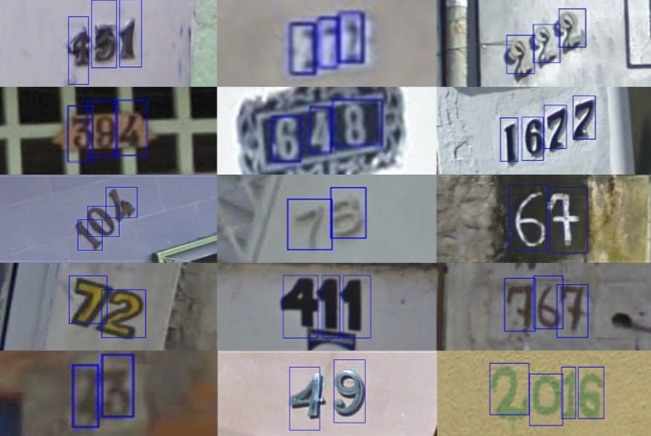
\includegraphics[width=\textwidth]{images/introduction/streetview}
    \caption{\footnotesize Localisation of digits found from varying street view house numbers using the worker described in \citet{Netzer:2011to}.}
  \end{subfigure} 
  \caption[Alphanumeric sequences observed in literature]{Various sample alphanumeric sequences observed in literature.}
  \label{fig:sample_sequences}
\end{figure}

\clearpage
\section{Motivation}
\label{sec:motivation}

Detection becomes difficult when the photo is unstructured. Early investigations in LPR systems were systematic in the subject material assessed; a detailed survey by \cite{Anagnostopoulos:2008vu} showed that they work best  with consistent lighting, specific colour and typeface detection, fixed detection regions, and non-noisy backgrounds. When applied in the context of images with unstructured backgrounds, these systematic approaches begin to have sever limitations as the text components cannot be easily determined.

While further investigations in the area utilise enhanced CC-based detection \citep{Chen:2011ul,Shivakumara:2011dl,Epshtein:2010tj}, performance is likely to degrade as image complexity increases \citep{Li:2012wd}. This is especially relevant when text is geometrically obfuscated, such as malformed RBNs as worn on a marathon runner's torso. Some studies have shown to overcome this by using facial recognition to find a more distinct candidate area \citep{Benami:2012jf}, but nonetheless relies on such properties like a person's face to detect a number. Similarly, most recognition techniques interpret text as segmented characters, rather than a single string, though there are exceptions such as in \cite{Zhu:2016ut}.
\section{Research Goals}
\label{sec:introduction:research_goals}

This study aims to develop a processing pipeline that both detects and recognises \glspl{rbn} on a marathon runner, and then ranks the prominence of each runner detected in the photo. The intention is to explore the viability of artificial deep-learning \glspl{nn}---such as \glspl{cnn}---in the pipeline. Previous studies in \gls{rbn} recognition \citep{Benami:2012jf} and similar areas \citep{Kundu:2015vq, Eichner:2008dw, Torresen:2004jl} were heavily heuristic and rule driven.

This primary aim is developed into three key objectives:

%By working with a large labelled dataset in the context of RBN recognition, a benchmark between existing libraries and open source tools can be assessed using techniques developed in other related works. A collated literature review of the state of the art in image processing and image segmentation from other similar areas (such as speed limit sign detection) is to be conducted. The study will also attempt to train a neural network to recognise entire numbers in an RBN, rather than segmented numbers joined together.

%When compared to the wider context of alphanumeric text recognition, this study focuses solely in the area of RBN detection. A generalised approach may be evolved from the study, such as applying the pipeline to other subjects or moving images (such as parked cars).


\subsubsection*{Goal 1: \itshape Detect \glspl{rbn} using a \gls{cnn}}

% 1: Explain the hypothesis
Literature has shown that heuristic-based detection algorithms (that are \gls{cc}-based) are able to detect text within photos \citep{Li:2012wd, Chen:2011ul, Eichner:2008dw}. We propose to apply these rule-based techniques to a large labelled dataset within the context of \glspl{rbn}, and contrast them against a learning-based detection and recognition algorithms (using \glspl{nn}). By benchmarking a against existing libraries and open source tools, we explore if heuristic-based detection algorithms (focusing namely on \gls{cc}-based detection) outperforms learning-based detection methods.
% 2: Suggest the research question from the hypothesis
For this goal the research question is framed as:
\begin{enumerate}[label=\bfseries~RQ\arabic*), leftmargin=2cm, rightmargin=1.5cm]
  \item\label{rq:1} Do \glspl{cnn} detect \glspl{rbn} with equal or higher recall and precision rates than \gls{cc}-based methods?
\end{enumerate}
% 3: Explain what phenomenon that will be observed
% 4: Explain possible evidence that shows this phenomenon
%The findings from these experiments offer metrics (namely, recall and precision rates) to compare the merit of learning-based versus \gls{cc}-based detection methods within our dataset of marathon photos. We observed that the precision and recall rates of learning-based detection methods compared \todo{favourably$~|~$worse than} those of \gls{cc}-based methods.

\subsubsection*{Goal 2: \itshape Design a \gls{cnn} that can recognise \glspl{rbn}}

% 1: Explain the hypothesis
Typically, traditional alphanumeric sequence parsing can be performed by character segmentation, and then piping those characters into \gls{ocr} engines.
% 2: Suggest the research question from the hypothesis
In the context of marathon photos, we explore answers to the following:
\begin{enumerate}[label=\bfseries~RQ\arabic*), leftmargin=2cm, rightmargin=1.5cm]
  \setcounter{enumi}{1}
  \item\label{rq:2} Does a \gls{cnn}-based \gls{ocr} approach outperform or is at parity with traditional \gls{ocr} approaches with higher or equal recall and precision rates?
  \item\label{rq:3} Does a \gls{cnn}-based \gls{ocr} algorithm perform \textit{without} the use of character segmentation?
\end{enumerate}
% 3: Explain what phenomenon that will be observed
% 4: Explain possible evidence that shows this phenomenon
% The findings from these experiments observed that the development of our learning-based \gls{ocr} pipeline outperformed that of a traditional \gls{ocr} engine by a factor of \todo{value}.

\subsubsection*{Goal 3: \itshape Rank prominence of alphanumeric sequences}

% 1: Explain the hypothesis
Our research objective is aimed to compare if humans are always better at ranking the prominence of an RBN than a \gls{nn}.
% 2: Suggest the research question from the hypothesis
We can therefore propose the followings research questions:
\begin{enumerate}[label=\bfseries~RQ\arabic*), leftmargin=2cm, rightmargin=1.5cm]
  \setcounter{enumi}{3}
  \item\label{rq:4} Can a deep-learning \gls{nn} be trained to rank marathon runners by prominence?, and if so
  \item\label{rq:5} Does a trained deep-learning \gls{nn} rank prominence of a runner better or equal to a human?
\end{enumerate}
% 3: Explain what phenomenon that will be observed
% 4: Explain possible evidence that shows this phenomenon
%The findings from these experiments observed that the development of a ranking system for \glspl{rbn} was able to match human characteristics with a similarity factor of \todo{value}.

\section{Thesis Organisation}

This thesis is organised into the chapters as outlined below. An appendix follows with additional supplementary material.

\paragraph{Chapter \ref{ch:background_work} - Background Work} Provides an overview of prior studies broadly around the areas of number recognition in image processing and artificial neural networks.

\paragraph{Chapter \ref{ch:related_work} - Related Work} Documents a number case studies within the literature directly or closely related to the aims of this research.

\paragraph{Chapter \ref{ch:research_methodology} - Research Methodology} Describes possible techniques in closer depth to develop a number recognition pipeline, and explores ways to develop prominence ranking techniques.

\paragraph{Chapter \ref{ch:benchmarking} - Benchmarking} Collates results of a series of experiments using our dataset amongst other tools and pipelines currently developed.

\paragraph{Chapter \ref{ch:processing_pipeline} - Processing Pipeline} Discusses the proposed processing pipeline developed that satisfies the aims of this study.

\paragraph{Chapter \ref{ch:deep_learning_comparison} - Deep Learning Comparison} Compares our deep-learning approach with those benchmarked.

\paragraph{Chapter \ref{ch:validation_of_results} - Validation of Results} Highlights a number of validation techniques used to ensure results found in the comparison are correct.

\paragraph{Chapter \ref{ch:discussion} - Discussion and Limitations}Presents implications that were found from the results of our findings and possible limitations.

\paragraph{Chapter \ref{ch:conclusion} - Conclusions and Future Work} Draws a number of conclusions and alleviates gaps in the findings of this work by presenting future studies.

\section*{Summary}

In this chapter we identified some shortcomings in text recognition, developed the context of the study---namely \gls{rbn} detection. We discussed the general stages that exist for text parsing within natural scenes, detection and recognition, and introduced typical techniques that are applied in this context. We outlined the research aims this study achieves, and how the thesis is organised. The following chapter will detail applications of image processing, using neural networks for image processing, and outline what techniques have been used in previous studies to achieve this.